% SC1007 — Chapter 1: Arrays, Linked Lists & Foundations
% No \documentclass — included by modules/SC1007/main.tex (book class).
\chapter{Arrays, Linked Lists \& Foundations}
\label{ch:stl-foundations}

\begin{quote}
\emph{``The machine can only store bits contiguously or linked by pointers.''} --- Every data structure trades off these two extremes.
\end{quote}

\noindent\textbf{Prerequisites:} SC1003 (C/Python basics). This chapter is the 0$\to$1: how data lives in memory and how STL wraps it.

\section*{Learning Outcomes}
After this chapter you will be able to:
\begin{enumerate}[label=(L\arabic*)]
    \item compare array vs.\ linked-list layouts and their $O(\cdot)$ costs;
    \item implement singly/doubly linked lists with invariants;
    \item analyse dynamic arrays (amortised doubling) and use STL \texttt{vector};
    \item choose the right sequential container and justify it.
\end{enumerate}

% ============================================================
\section{Contiguous Storage: Arrays}
% --- Chapter 1 content begins ---
\label{sec:arrays}
A \emph{pointer} is a variable whose value is a memory address; dereferencing follows the address to the stored object. Asymptotic costs: $f(n)=\Theta(g(n))$ means $c_{1}g(n)\le f(n)\le c_{2}g(n)$ for large $n$ (tight bound), $O(g)$ is an upper bound, $\Omega(g)$ a lower bound. $O(1)$ = constant time independent of $n$; $O(n)$ = linear in $n$.

An \emph{array} stores $n$ elements consecutively. If base address is $B$ and each element occupies $w$ bytes,
\begin{equation}
\text{addr}(A[i]) = B + i\cdot w,
\label{eq:array-addr}
\end{equation}
so random access is $\Theta(1)$. Insertion/deletion at position $k$ shifts $n-k$ elements: $\Theta(n)$.

\textbf{Static vs.\ dynamic.} Static arrays have fixed capacity. A \emph{dynamic array} (C++ \texttt{vector}, Java \texttt{ArrayList}, Python \texttt{list}) doubles capacity when full. Appending $n$ items costs $O(n)$ total --- amortised $O(1)$ per append.

\begin{figure}[h]
\centering
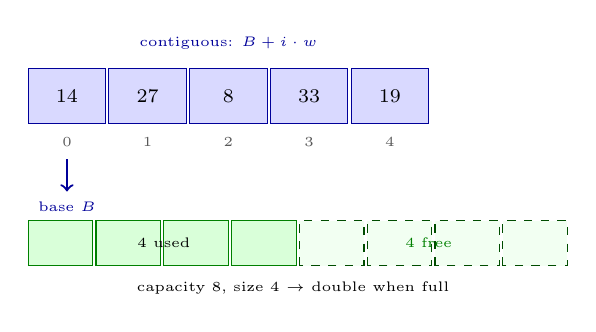
\begin{tikzpicture}[scale=0.82, every node/.style={font=\scriptsize}]
  \foreach \i/\v in {0/14,1/27,2/8,3/33,4/19} {
    \draw[fill=blue!15, draw=blue!60!black] (\i*1.25,0) rectangle ++(1.2,0.85);
    \node at (\i*1.25+0.6,0.42) {\v};
    \node[font=\tiny, gray!70!black] at (\i*1.25+0.6,-0.28) {\i};
  }
  \node[font=\tiny, blue!60!black] at (3.1,1.25) {contiguous: $B+i\cdot w$};
  \draw[->, blue!60!black, thick] (0.6,-0.55) -- ++(0,-0.5) node[below, font=\tiny] {base $B$};
  \begin{scope}[yshift=-2.2cm]
    \foreach \i in {0,1,2,3} {
      \draw[fill=green!15, draw=green!50!black] (\i*1.05,0) rectangle ++(1.0,0.7);
    }
    \foreach \i in {4,5,6,7} {
      \draw[fill=green!5, draw=green!30!black, dashed] (\i*1.05,0) rectangle ++(1.0,0.7);
    }
    \node at (2.1,0.35) {\tiny 4 used};
    \node[font=\tiny, green!50!black] at (6.2,0.35) {4 free};
    \node[font=\tiny] at (4.1,-0.35) {capacity 8, size 4 $\to$ double when full};
  \end{scope}
\end{tikzpicture}
\caption{Array in memory (top): index $\to$ address in $O(1)$. Dynamic array (bottom): doubling gives amortised $O(1)$ append.}
\label{fig:array-layout}
\end{figure}

\begin{lstlisting}[language=C++]
// C++ STL vector -- dynamic array
#include <vector>
std::vector<int> v = {14, 27, 8};
v.push_back(33);            // amortised O(1)
int x = v[1];               // O(1) random access
v.insert(v.begin()+1, 99);  // O(n) -- shifts right
\end{lstlisting}

% ============================================================
\section{Linked Storage: Linked Lists}
\label{sec:linked-lists}
A \emph{linked list} scatters nodes; each node holds data plus pointer(s) to neighbours. No shifting is needed for mid-list insertion.

\begin{definition}[Singly linked list]
A chain $p_{0}\to p_{1}\to\cdots\to p_{n-1}\to\texttt{null}$ where node $p_{i}$ stores $(x_{i}, \texttt{next})$. Doubly linked adds $\texttt{prev}$.
\end{definition}

\begin{figure}[h]
\centering
\begin{tikzpicture}[scale=0.85, every node/.style={font=\scriptsize},
  llnode/.style={draw, thick, fill=orange!15, minimum width=1.7cm, minimum height=0.85cm, rounded corners=2pt},
  ptr/.style={-{Stealth}, thick, blue!60!black}]
  \node[llnode] (n0) at (0,0) {14 \quad $\mid$ \quad $\bullet$};
  \node[llnode] (n1) at (3,0) {27 \quad $\mid$ \quad $\bullet$};
  \node[llnode] (n2) at (6,0) {8 \quad $\mid$ \quad $\bullet$};
  \node (null) at (9.2,0) {null};
  \draw[ptr] (n0.east) -- (n1.west);
  \draw[ptr] (n1.east) -- (n2.west);
  \draw[ptr] (n2.east) -- (null.west);
  \node[above, font=\tiny, blue!60!black] at (1.5,0.55) {next};
  \begin{scope}[yshift=-1.8cm, xshift=1.5cm]
    \node[draw, fill=violet!12, minimum width=1.9cm, minimum height=0.75cm, rounded corners=2pt, font=\scriptsize] (d0) at (0,0) {$\bullet\mid 14\mid\bullet$};
    \node[draw, fill=violet!12, minimum width=1.9cm, minimum height=0.75cm, rounded corners=2pt, font=\scriptsize] (d1) at (3.2,0) {$\bullet\mid 27\mid\bullet$};
    \draw[{Stealth}-{Stealth}, thick, violet!70!black] (d0.east) -- (d1.west);
    \node[font=\tiny, violet!70!black] at (1.6,0.55) {prev / next};
    \node[font=\tiny, gray!60!black] at (1.6,-0.65) {doubly: $O(1)$ delete given node ptr};
  \end{scope}
\end{tikzpicture}
\caption{Singly linked list (top) vs.\ doubly linked fragment (bottom). Pointer chasing replaces index arithmetic.}
\label{fig:linked-list}
\end{figure}

Operations: access by index $\Theta(n)$ (must walk); insert/delete at head $\Theta(1)$; after locating position $k$, pointer rewiring is $\Theta(1)$. Doubly linked allows $O(1)$ deletion given a node pointer.

\begin{lstlisting}[language=Python]
# Linked list node -- Python
class Node:
    def __init__(self, val, nxt=None):
        self.val = val
        self.next = nxt

def insert_after(node, val):
    node.next = Node(val, node.next)  # O(1)

def delete_after(node):
    if node.next:
        node.next = node.next.next   # O(1)
\end{lstlisting}

% ============================================================
\section{Complexity Comparison \& STL Choice}
\label{sec:comparison}

\begin{table}[h]
\centering
\small
\begin{tabular}{lcc}
\toprule
Operation & Array / \texttt{vector} & Linked list \\
\midrule
Access $A[k]$ & $\Theta(1)$ & $\Theta(n)$ \\
Append at end & amort.\ $\Theta(1)$ & $\Theta(1)^{*}$ \\
Insert at $k$ & $\Theta(n-k)$ shift & $\Theta(k)$ seek $+$ $\Theta(1)$ link \\
Delete at $k$ & $\Theta(n-k)$ shift & $\Theta(k)$ seek $+$ $\Theta(1)$ link \\
Memory overhead & low (contiguous) & $+1$--$2$ ptrs / elem \\
\bottomrule
\end{tabular}
\caption{Sequential containers compared. $^{*}$With tail pointer; else $\Theta(n)$.}
\label{tab:seq-compare}
\end{table}

Rule of thumb: prefer \texttt{vector} unless you need frequent mid-list splicing with iterators or non-contiguous growth without reallocation.

\begin{figure}[h]
\centering
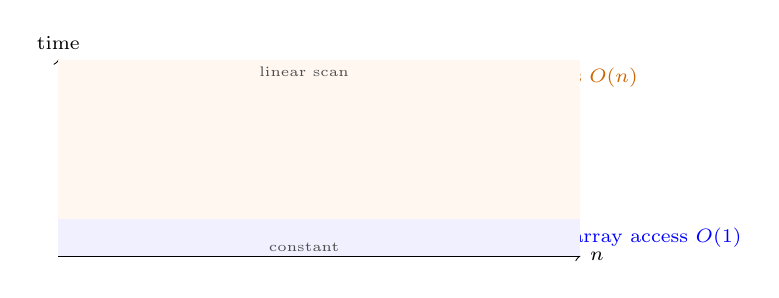
\begin{tikzpicture}[scale=0.78, every node/.style={font=\scriptsize}]
  \draw[->] (0,0) -- (8.5,0) node[right] {$n$};
  \draw[->] (0,0) -- (0,3.2) node[above] {time};
  \draw[blue, thick] (0,0.3) -- (8.2,0.3) node[right] {array access $O(1)$};
  \draw[orange!80!black, thick] plot[domain=0.2:8.2, smooth] (\x,{0.3+0.32*\x});
  \node[orange!80!black] at (8.2,2.9) {list access $O(n)$};
  \fill[blue!6] (0,0) rectangle (8.5,0.6);
  \fill[orange!6] (0,0.6) rectangle (8.5,3.2);
  \node[font=\tiny, gray!60!black] at (4,0.15) {constant};
  \node[font=\tiny, gray!60!black] at (4,3.0) {linear scan};
\end{tikzpicture}
\caption{Random access: array stays flat; linked list grows linearly with $n$.}
\label{fig:access-cost}
\end{figure}

% ============================================================

% --- Additional: STL iterators & amortised doubling proof sketch ---
\section{Iterators \& Amortised Doubling}
\label{sec:iterators-amortised}
STL decouples containers from algorithms via \emph{iterators}. A vector iterator is a random-access pointer; a list iterator is bidirectional. Algorithms like \texttt{std::sort} require random access, so they work on vectors but not lists.

\textbf{Amortised doubling proof.} Start with capacity $1$. Insert $n$ items, doubling when full. Total copies:
\begin{equation}
1+2+4+\cdots+2^{\lceil\log_{2}n\rceil-1} < 2n.
\end{equation}
So $n$ appends cost $O(n)$ and average $O(1)$. Halving when size $<$ capacity$/4$ keeps both push and pop amortised $O(1)$ without thrashing.

\begin{lstlisting}[language=C++]
// Iterator example -- same code works for vector and deque
#include <vector>
#include <algorithm>
std::vector<int> v = {5,2,9,1,7};
std::sort(v.begin(), v.end()); // requires random-access iterators
for (auto it = v.begin(); it != v.end(); ++it) *it += 1;
\end{lstlisting}

\begin{remark}
Python \texttt{list} over-allocates similarly; CPython grows by $\approx 1.125\times$ for large lists. Java \texttt{ArrayList} grows by $1.5\times$. Constants affect memory but not the $O(1)$ amortised bound.
\end{remark}

\section{Chapter Notes}
CLRS Ch.~10, Weiss Ch.~3. STL: \texttt{vector} is dynamic array; \texttt{list} is doubly linked; \texttt{deque} is in Ch.~2. Python \texttt{list} is a dynamic array, not a linked list.

% ============================================================
\section{Exercises}
\label{sec:ch01-exercises}
\begin{enumerate}[label=E1.\arabic*, leftmargin=*, itemsep=0.7em]
    \item \textbf{Address arithmetic.} Array \texttt{int A[100]} at base $B=0x1000$, $w=4$ bytes. (a) Address of \texttt{A[37]}? (b) Why does \texttt{A[i][j]} in $m\times n$ row-major cost $B+(i\cdot n+j)w$?
    \item \textbf{Doubling analysis.} Starting from capacity $1$, insert $n=2^{k}$ items with doubling. Count total element copies. Show it is $<2n$ and deduce amortised $O(1)$.
    \item \textbf{Linked list reversal.} Write iterative $O(n)$-time $O(1)$-space reversal for singly linked list. Prove your loop invariant: after $t$ iterations the prefix of length $t$ is reversed.
    \item \textbf{Container choice.} For each scenario choose \texttt{vector} vs.\ \texttt{list} and justify: (a) 1M insertions at random positions with iterator kept; (b) binary search over sorted data; (c) queue with push/pop at ends only.
    \item \textbf{Splice.} Given doubly linked list with head/tail, splice node $x$ (in $L_{1}$) into $L_{2}$ after node $y$ in $O(1)$. Give pointer updates and handle head/tail edge cases.
\end{enumerate}
% End of Chapter 1 — amortised analysis bridges to Ch.~8 recurrences.
